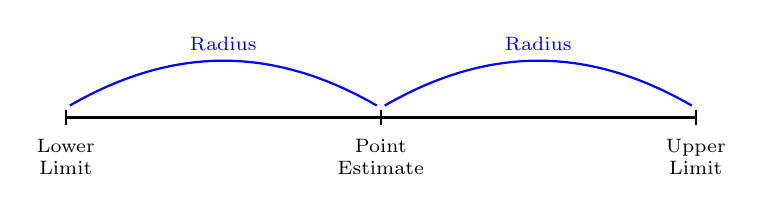
\begin{tikzpicture}
  \draw[thick] (0,0) -- (8,0);
  \foreach \i in {0,4,8} {
      \draw[thick] (\i,0.1) -- (\i,-0.1);
  };
  \node[align=center,execute at begin node=\setlength{\baselineskip}{0.8em}] at (0,-0.5) {
      \scriptsize Lower\\ \scriptsize Limit
  };
  \node[align=center,execute at begin node=\setlength{\baselineskip}{0.8em}] at (4,-0.5) {
    \scriptsize Point\\ \scriptsize Estimate
  };
  \node[align=center,execute at begin node=\setlength{\baselineskip}{0.8em}] at (8,-0.5) {
    \scriptsize Upper\\ \scriptsize Limit
  };
  \draw[blue,thick] (0.05,0.15) to [bend left] node[midway,above] {\scriptsize Radius} (3.95,0.15);
  \draw[blue,thick] (4.05,0.15) to [bend left] node[midway,above] {\scriptsize Radius} (7.95,0.15);
\end{tikzpicture}